\documentclass{article}
\usepackage[UTF8]{ctex}
\usepackage{mathtools,amsmath,geometry,enumerate,float}

\geometry{a4paper,scale=0.8}

\newcommand\bo[1]{\boldsymbol{#1}}
\renewcommand\v[1]{\overrightarrow{#1}}

\usepackage{pgfplots}
\pgfplotsset{compat=1.15}
\usepackage{mathrsfs}
\usetikzlibrary{arrows}
\pagestyle{empty}

\title{2024TST P2}
\author{}
\date{}

\begin{document}
\textbf{题目(2024 CTST P2):}\par
{\kaishu 在锐角$\triangle ABC$中, $\angle A>\angle B>\angle C$. $B_1, C_1$是平面上的两点, 满足$\triangle AC_1B$和$\triangle CB_1A$分别是以$AB,AC$为底边, 且顺相似的等腰三角形. 设直线$BB_1,CC_1$交于点$T$. 假设上述各点两两不同, 求证: $\angle ATC\neq 90^\circ$.}\par 
\begin{figure}[H]
	\centering 
	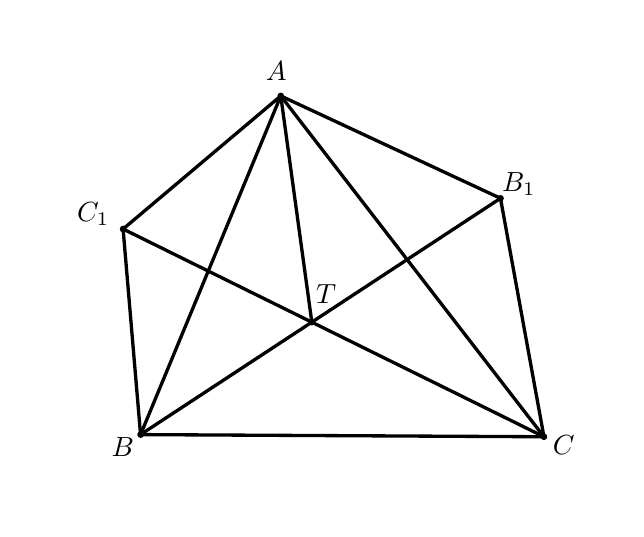
\begin{tikzpicture}[line cap=round,line join=round,>=triangle 45,x=1.0cm,y=1.0cm]
		\clip(-2.0032470777096876,-2.304171781561702) rectangle (5.466904311783417,3.8121972831080106);
		\draw [line width=1.2pt] (1.2111199031710533,2.945265514258693)-- (-0.5695841731129752,-1.3558197161504217);
		\draw [line width=1.2pt] (-0.5695841731129752,-1.3558197161504217)-- (4.553364477119538,-1.3832151634778684);
		\draw [line width=1.2pt] (4.553364477119538,-1.3832151634778684)-- (1.2111199031710533,2.945265514258693);
		\draw [line width=1.2pt] (-0.7913099657729439,1.2551372876027274)-- (1.2111199031710533,2.945265514258693);
		\draw [line width=1.2pt] (-0.7913099657729439,1.2551372876027274)-- (-0.5695841731129752,-1.3558197161504217);
		\draw [line width=1.2pt] (4.001403319232643,1.6451875662046929)-- (1.2111199031710533,2.945265514258693);
		\draw [line width=1.2pt] (4.001403319232643,1.6451875662046929)-- (4.553364477119538,-1.3832151634778684);
		\draw [line width=1.2pt] (-0.7913099657729439,1.2551372876027274)-- (4.553364477119538,-1.3832151634778684);
		\draw [line width=1.2pt] (4.001403319232643,1.6451875662046929)-- (-0.5695841731129752,-1.3558197161504217);
		\draw [line width=1.2pt] (1.6053055906744635,0.07206868441407377)-- (1.2111199031710533,2.945265514258693);
		
		\draw [fill=black] (1.2111199031710533,2.945265514258693) circle (1.0pt);
		\draw[color=black] (1.1523318664829665,3.261918856111452) node {$A$};
		\draw [fill=black] (-0.5695841731129752,-1.3558197161504217) circle (1.0pt);
		\draw[color=black] (-0.7955563706729928,-1.5104073249206489) node {$B$};
		\draw [fill=black] (4.553364477119538,-1.3832151634778684) circle (1.0pt);
		\draw[color=black] (4.804622311150391,-1.4909284425490892) node {$C$};
		\draw [fill=black] (-0.7913099657729439,1.2551372876027274) circle (1.0pt);
		\draw[color=black] (-1.170524856325515,1.4455130749635197) node {$C_1$};
		\draw [fill=black] (4.001403319232643,1.6451875662046929) circle (1.0pt);
		\draw[color=black] (4.234865001782273,1.8253512812089319) node {$B_1$};
		\draw [fill=black] (1.6053055906744635,0.07206868441407377) circle (1.0pt);
		\draw[color=black] (1.7880011317008554,0.427741471049531) node {$T$};
	
	\end{tikzpicture}
\end{figure}

解: 如图, 作点$A_1$, 使得$\triangle BA_1C\sim\triangle AC_1B$.

\begin{figure}[H]
	\centering 
	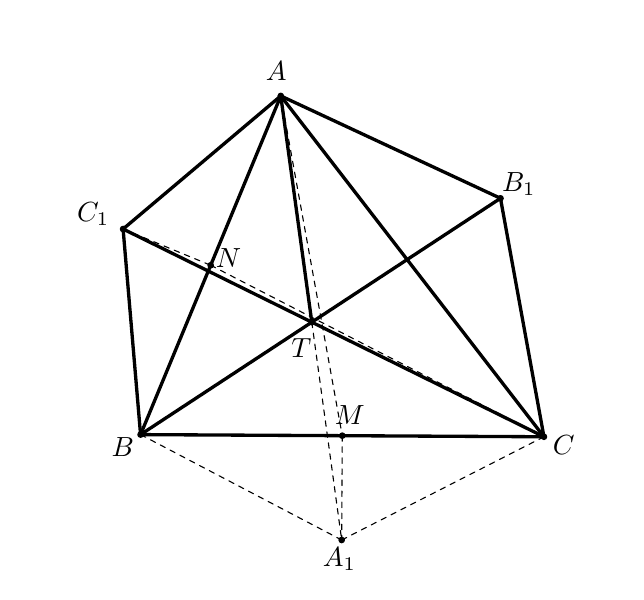
\begin{tikzpicture}[line cap=round,line join=round,>=triangle 45,x=1.0cm,y=1.0cm]
		\clip(-2.0032470777096876,-3.104171781561702) rectangle (5.466904311783417,3.8121972831080106);
		\draw [line width=1.2pt] (1.2111199031710533,2.945265514258693)-- (-0.5695841731129752,-1.3558197161504217);
		\draw [line width=1.2pt] (-0.5695841731129752,-1.3558197161504217)-- (4.553364477119538,-1.3832151634778684);
		\draw [line width=1.2pt] (4.553364477119538,-1.3832151634778684)-- (1.2111199031710533,2.945265514258693);
		\draw [line width=1.2pt] (-0.7913099657729439,1.2551372876027274)-- (1.2111199031710533,2.945265514258693);
		\draw [line width=1.2pt] (-0.7913099657729439,1.2551372876027274)-- (-0.5695841731129752,-1.3558197161504217);
		\draw [line width=1.2pt] (4.001403319232643,1.6451875662046929)-- (1.2111199031710533,2.945265514258693);
		\draw [line width=1.2pt] (4.001403319232643,1.6451875662046929)-- (4.553364477119538,-1.3832151634778684);
		\draw [line width=0.4pt,dash pattern=on 2pt off 2pt] (1.9848068537179184,-2.694094219177017)-- (-0.5695841731129752,-1.3558197161504217);
		\draw [line width=0.4pt,dash pattern=on 2pt off 2pt] (1.9848068537179184,-2.694094219177017)-- (4.553364477119538,-1.3832151634778684);
		\draw [line width=1.2pt] (-0.7913099657729439,1.2551372876027274)-- (4.553364477119538,-1.3832151634778684);
		\draw [line width=1.2pt] (4.001403319232643,1.6451875662046929)-- (-0.5695841731129752,-1.3558197161504217);
		\draw [line width=1.2pt] (1.6053055906744635,0.07206868441407377)-- (1.2111199031710533,2.945265514258693);
		\draw [line width=0.4pt,dash pattern=on 2pt off 2pt] (1.6053055906744635,0.07206868441407377)-- (1.9848068537179184,-2.694094219177017);
		\draw [line width=0.4pt,dash pattern=on 2pt off 2pt] (-0.7913099657729439,1.2551372876027274)-- (0.3207678650290391,0.7947228990541356);
		\draw [line width=0.4pt,dash pattern=on 2pt off 2pt] (0.3207678650290391,0.7947228990541356)-- (4.553364477119538,-1.3832151634778684);
		\draw [line width=0.4pt,dash pattern=on 2pt off 2pt] (1.2111199031710533,2.945265514258693)-- (1.9918901520032812,-1.3695174398141452);
		\draw [line width=0.4pt,dash pattern=on 2pt off 2pt] (1.9918901520032812,-1.3695174398141452)-- (1.9848068537179184,-2.694094219177017);
		
		\draw [fill=black] (1.2111199031710533,2.945265514258693) circle (1.0pt);
		\draw[color=black] (1.1523318664829665,3.261918856111452) node {$A$};
		\draw [fill=black] (-0.5695841731129752,-1.3558197161504217) circle (1.0pt);
		\draw[color=black] (-0.7955563706729928,-1.5104073249206489) node {$B$};
		\draw [fill=black] (4.553364477119538,-1.3832151634778684) circle (1.0pt);
		\draw[color=black] (4.804622311150391,-1.4909284425490892) node {$C$};
		\draw [fill=black] (-0.7913099657729439,1.2551372876027274) circle (1.0pt);
		\draw[color=black] (-1.170524856325515,1.4455130749635197) node {$C_1$};
		\draw [fill=black] (4.001403319232643,1.6451875662046929) circle (1.0pt);
		\draw[color=black] (4.234865001782273,1.8253512812089319) node {$B_1$};
		\draw [fill=black] (1.9848068537179184,-2.694094219177017) circle (1.0pt);
		\draw[color=black] (1.9558357643097999,-2.937235458637389) node {$A_1$};
		\draw [fill=black] (1.6053055906744635,0.07206868441407377) circle (1.0pt);
		\draw[color=black] (1.4737334256136998,-0.25401941195505484) node {$T$};
		\draw [fill=black] (0.3207678650290391,0.7947228990541356) circle (1.0pt);
		\draw[color=black] (0.5484865129646193,0.8854952067811814) node {$N$};
		\draw [fill=black] (1.9918901520032812,-1.3695174398141452) circle (1.0pt);
		\draw[color=black] (2.0873182203178273,-1.1110902363036772) node {$M$};

	\end{tikzpicture}
\end{figure}
设$\triangle ABC$的内角为$A,B,C$, 三个等腰三角形的底角为$\alpha$. 则由正弦定理,
\[\frac{\sin\angle TAB}{\sin\angle TAC}=\frac{A_1B\cdot\sin\angle ABA_1/AA_1}{A_1C\cdot\sin\angle ACA_1/AA_1}=\frac{\sin\angle ABA_1}{\sin\angle ACA_1}=\frac{\sin(B+\alpha)}{\sin(C+\alpha)}.\]
则
\[\prod_{\mathrm{cyc}}\frac{\sin{\angle TAB}}{\sin{\angle TAC}}=\prod_{\mathrm{cyc}}\frac{\sin(B+\alpha)}{\sin(C+\alpha)}=1.\]
由角元塞瓦定理, 知$AA_1, BB_1,CC_1$共点.\par 
作$BC, AB$中点$M,N$, 则$MA_1\perp BC, NC_1\perp AB$. 记垂直于纸面的向外的单位向量为$\bo{e}$, 设$k=MA_1/BC$($A, A_1$在直线$BC$异侧时$k>0$, 否则$k<0$). 并且设$\triangle ABC$的三边为$a,b,c$, 面积为$S$, 则由 $\angle A>\angle B>\angle C$知$a>b>c>0$, 且
\[\v{AA_1}=\v{AM}+\v{,MA_1}=\v{AM}+k\v{BC}\times\bo e,\v{CC_1}=\v{CN}+k\v{AB}\times\bo e.\]
则
\begin{align*}
\v{AA_1}\cdot\v{CC_1}&=(\v{AM}+k\v{BC}\times\bo e)\cdot (\v{CN}+k\v{AB}\times\bo e)\\
&=\frac14(\v{AB}+\v{AC})\cdot(\v{CA}+\v{CB})+k\v{AM}\cdot(\v{AB}\times\bo{e})+k\v{CN}\cdot(\b{BC}\times\bo e)+k^2(\v{BC}\times\bo e)\cdot(\v{AB}\times\bo e). 
\end{align*}
由点乘、叉乘的性质,
\[\v{AM}\cdot(\v{AB}\times\bo{e})=2S_{\triangle AMB},\v{CN}\cdot(\v{BC}\times\bo e)=2S_{\triangle NBC},\]
\[(\v{BC}\times\bo e)\cdot(\v{AB}\times\bo e)=\v{BC}\cdot\v{AB}.\]
故
\begin{align*}
&\frac14(\v{AB}+\v{AC})\cdot(\v{CA}+\v{CB})+k\v{AM}\cdot(\v{AB}\times\bo{e})+k\v{CN}\cdot(\b{BC}\times\bo e)+k^2(\v{BC}\times\bo e)\cdot(\v{AB}\times\bo e)\\
=&-\frac14\v{AB}\cdot\v{AC}+\frac14\v{BA}\cdot\v{BC}-\frac14AC^2-\frac14\v{CA}\cdot\v{CB}+2k(S_{\triangle AMB}+S_{\triangle NBC})-k^2\v{BC}\cdot\v{BA}\\
=&-\frac18(b^2+c^2-a^2)+\frac18(a^2+c^2-b^2)-\frac18(a^2+b^2-c^2)-\frac{b^2}{4}+2kS-\frac{k^2}{2}(a^2+c^2-b^2)\\
=&-\frac{a^2+c^2-b^2}{2}k^2+2S\cdot k-\frac{5b^2-a^2-c^2}{8}
.\end{align*}
这是一个关于$k$的二次函数, 其判别式为
\begin{align*}
&(2S)^2-4\frac{a^2+c^2-b^2}{2}\frac{5b^2-a^2-c^2}{8}\\
=&\frac14\left(16S^2-(a^2+c^2-b^2)(5b^2-a^2-c^2)\right)\\
=&\frac14\left(2\sum_{\mathrm{cyc}}a^2b^2-\sum_{\mathrm{cyc}}a^4-(a^2+c^2-b^2)(5b^2-a^2-c^2)\right)\\
=&-\left(a^2-b^2\right)\left(b^2-c^2\right)<0.
\end{align*}
故对任意的实数$k$, $\v{AA_1}\cdot\v{CC_1}$均不为$0$. 证毕!
\end{document}